% generation d'un .a que tu peux utiliser en ajoutant USE_STATIC_LIB=1 dans ton Makefile
% ajouter LDFLAGS+=-liio dans Makefile cree par module_generator

% device_reboot sf
% dfu-util -a firmware.dfu -D pluto.dfu

% dans le .dts : on remplace target = <&fpga_full>; par target = <&fpga_axi>; et on commente le nom du bitstream

\documentclass{article}
\usepackage{makeidx,anysize,mflogo,xspace,float,epsfig,url}
\usepackage{amsmath,amsfonts,amssymb,a4wide,fullpage} 
%\usepackage[francais]{babel}
%\usepackage[french]{babel}
\urlstyle{sf}
%\usepackage{subcaption}
\usepackage{hyperref}
\usepackage{graphicx}
\usepackage{graphics}
\usepackage{float}
\usepackage{caption}
\usepackage{colordvi} %??
\usepackage{listings} 
\usepackage{subfigure}
\usepackage{subfloat}
\usepackage{xcolor}
\graphicspath{{./images/}}
%\usepackage[labelsep=quad,indention=10pt]{subfig}
\definecolor{grey}{rgb}{0.95,0.95,0.95} 
	\definecolor{red}{rgb}{1.0,0.0,0.0} 
	\definecolor{green}{rgb}{0.0,0.7,0.0}
	\definecolor{blue}{rgb}{0.0,0.0,1.0}
	\lstloadlanguages{bash,Java,C,C++,csh,make,sh}%%[Visual]Basic,xml}
	\lstset{frame=none,basicstyle=\footnotesize,breaklines,tabsize=2,captionpos=b,
		prebreak={\hbox{$\rightarrow$}},postbreak={\hbox{$\hookrightarrow$}},
		showstringspaces=false,backgroundcolor=\color{grey}\bfseries,
		keywordstyle=\color{blue},commentstyle=\color{green}\textit,
		stringstyle=\color{red}\ttfamily,abovecaptionskip=2pt,aboveskip=0pt,
		belowskip=0pt,belowcaptionskip=0pt,numbers=none,columns=fullflexible, backgroundcolor=\color{grey}}
%left,numberstyle=\footnotesize,
%		stepnumber=2,numbersep=1pt}

\begin{document}


\begin{center}
{\bf \Large Decoding GPS signals using ADALM-PLUTO within \\ the OscimpDigital Ecosystem} \\ \ \\
G. Goavec-Merou, J.-M Friedt \\ {\tt \{gwenhael.goavec,jmfriedt\}@femto-st.fr}\ \\ \today
\end{center}

This tutorial is intended to demonstrate the use of the OSCIMP framework to generate
a bitstream in the ADALM-PLUTO programmable logic part of the Zynq CPU to decode GPS \cite{collins} signals.
It focuses on

\begin{itemize}
	\item Introducing basics of GPS and CDMA communication
	\item Introducing basics of Pseudo Random Number (PRN) generator and demonstrating some CDMA basics
	\item Introducing means of correcting carrier frequency differences between emitter and receiver and how to compensate
for such differences in a context of binary phase shift keying (phase modulation)
	\item Demonstrating GPS decoding by running all identifiers over all possible Doppler frequency shifts
\end{itemize}

The new processing blocks introduced in this tutorial are the 7-bit PRN generator, GPS Gold Code 
PRN generator, complex mixer and correlator.

\begin{figure}[h!]
\begin{center}
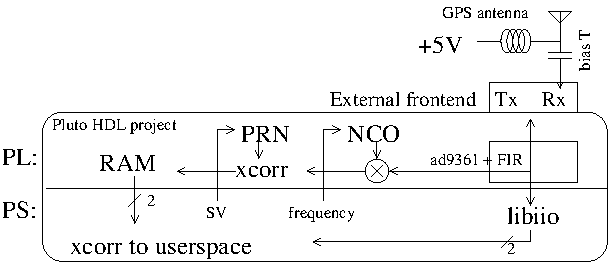
\includegraphics[width=.7\linewidth]{pluto-oscimpDigital-objective}
\end{center}
\caption{Objectives of this tutorial and raw schematics of the
processing chains. Decoding GPS requires being able to configure from the PS the Space Vehicle (SV)
number, defining which PRN Gold Code is generated, as well as the frequency offset to compensate for 
Doppler shift induced by satellite motion along its orbit.}
\end{figure}

The satellites of the GPS constellation all emit on the same carrier frequency of 1575.42~MHz. The
way the signal coming from each satellite is separated is by cross-correlating with each unique
satellite identifier, as classically done in Code Division Multiple Access. Correlating is 
a computationally intensive task either efficiently implemented through a Fast Fourier
Transform (converting a $N^2$ complexity algorithm to a $N\ln(N)$ complexity task) or parallelized
in an FPGA. 

Indeed, remembering that the correlation $xcorr()$ between $x$ and $y$ is expressed as
$$xcorr(x,y)(\tau)=\int x(t)y(t+\tau)dt\underbrace{\longrightarrow}_{discrete}xcorr(x,y)_n=\sum_k x_ny_{n+k}$$
and based on the convolution theorem, then 
$$FFT(xcorr(x,y))=FFT(x)\cdot FFT^*(y)\Leftrightarrow
xcorr(x,y)=iFFT\left(FFT(x)\cdot FFT^*(y)\right)$$ where $^*$ is the complex conjugate.

In this tutorial, we wish to demonstrate how the PlutoSDR firmware can be updated 
to include the Pseudo Random Number (PRN) generator identifying each satellite, how Doppler
shift can be compensated for by programming a numerically controlled oscillator without changing
the radiofrequency receiver local oscillator on-board the AD9363, and how cross-correlation is
computed on the programmable logic to only provide the processed data to the processing system
for display.

Rather than addressing immediately the complete GPS signal processing chain, we consider each
task sequentially by first demonstrating cross-correlation with a more simple 7-bit (127-long
sequence) PRN, show that the correlator is working properly on this simple signal when the emitter
and receiver carrier are at the same frequency (demonstration of code decoding and code 
orthogonality). Since GPS signals are emitted by satellites moving around the Earth at an
altitude of 20000~km inducing a Doppler shift of $\pm$5~kHz at 1575.42~MHz in addition to the
local oscillator offset, the emitter and receiver carrier frequency offset compensation is
demonstrated by adding in the programmable logic of the Zynq a numerically controlled oscillator
and a mixer. Having demonstrated these two basic steps, the 7-bit PRN generator is replaced
with the GPS 10-bit Gold Code generator and the cross-correlator block extended to process
1023-bit long sequences. The final result is a set of PRN-Doppler maps in which strong cross-correlation
demonstrate GPS signal decoding.

\section{7-bit PRN on the same receive and transmit carrier frequencies}

The first example aims at demonstrating the generation of an 7-bit long PRN sequence on the
Zynq Programmable Logic (PL) and correlating a transmitted signal modulated with such a sequence.
The PlutoSDR is fed by a signal generated from GNU Radio phase-modulating the carrier by
a GLFSR block configured to generate a known sequence. First of all, we become convinced of the 
accuracy of computing the cross-correlation as the inverse Fourier transform of the 
product of two Fourier transforms. Notice (Fig. \ref{f0}, left) that in order to have 0-delay in the middle 
of the time-domain chart and the negative delay to the left, we first compute two {\em inverse} Fourier 
transforms and the take the {\em direct} Fourier transform of their product. Fig. \ref{f0} (right) indeed exhibits
correlation peaks separated by the PRN repetition length -- 127 for an 7-bit PRN -- with a weighing dependent on
the windowing filter.

\begin{figure}[h!tb]
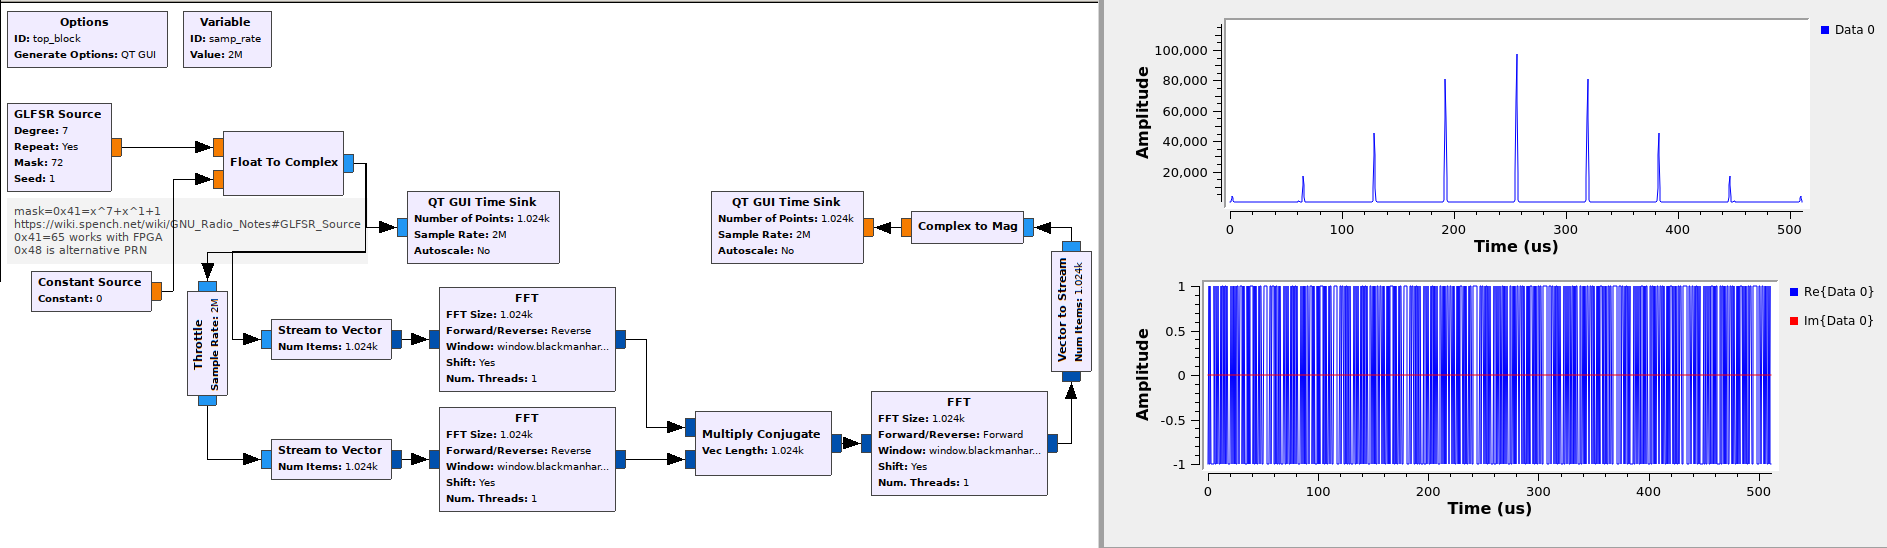
\includegraphics[width=\linewidth]{xcorr_pluto1.png}
\caption{Synthetic signal cross correlation demonstration}
\label{f0}
\end{figure}

The synthetic data example (Fig. \ref{f0}) is expanded by running on the PlutoSDR transceiver (Fig. \ref{f1}). In
that case, the BPSK modulation is created by running the output of the GLFSR block, with values either +1 or -1
with the pseudo-random sequence, as input of the PlutoSDR sink. Since $+1=\exp(j0)$ et $-1=\exp(j\pi)$, indeed
the resulting carrier modulation is a constant amplitude and phase shifting from $0$ to $\pi$, as expected
from BPSK. The PlutoSDR Source is then run through the same correlation scheme fed on the other side by the 
phase sequence generated by the GLFSR. The PlutoSDR output is connected to the PlutoSDR input through an optional
10~dB attenuator to reduce risks of damaging the radiofrequency input frontend (Fig. \ref{f1}, top).

\begin{figure}[h!tb]
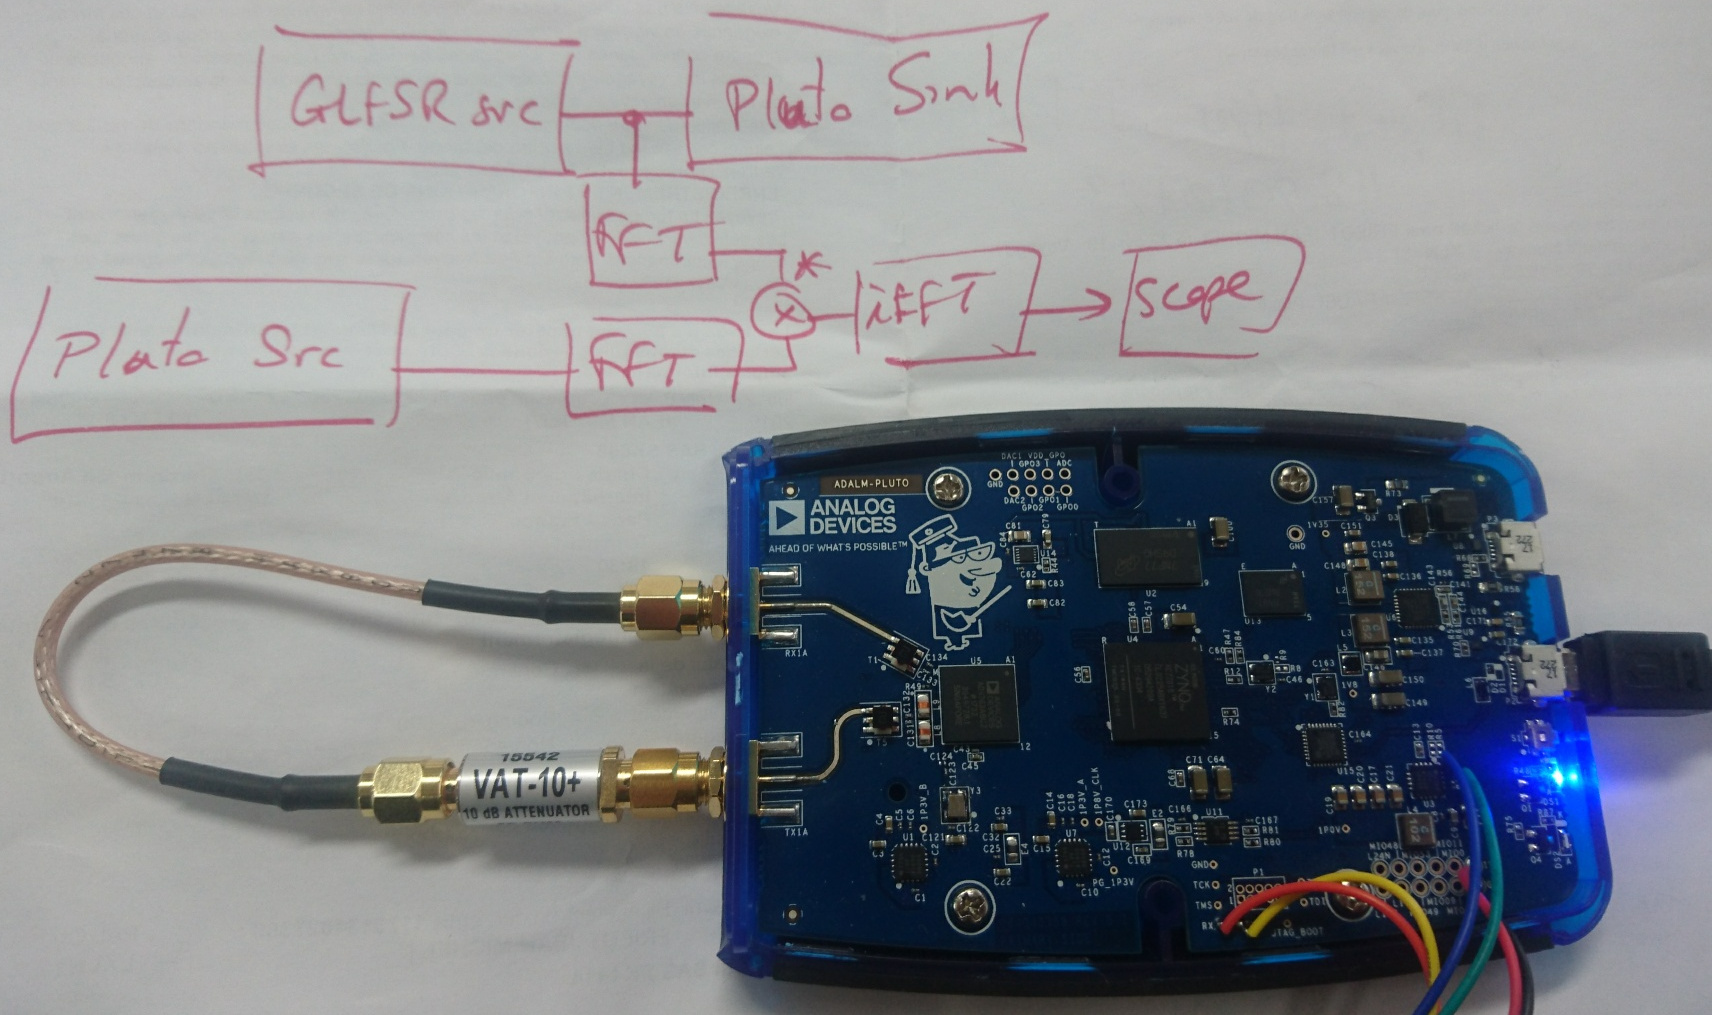
\includegraphics[width=\linewidth]{DSC_0275.JPG}
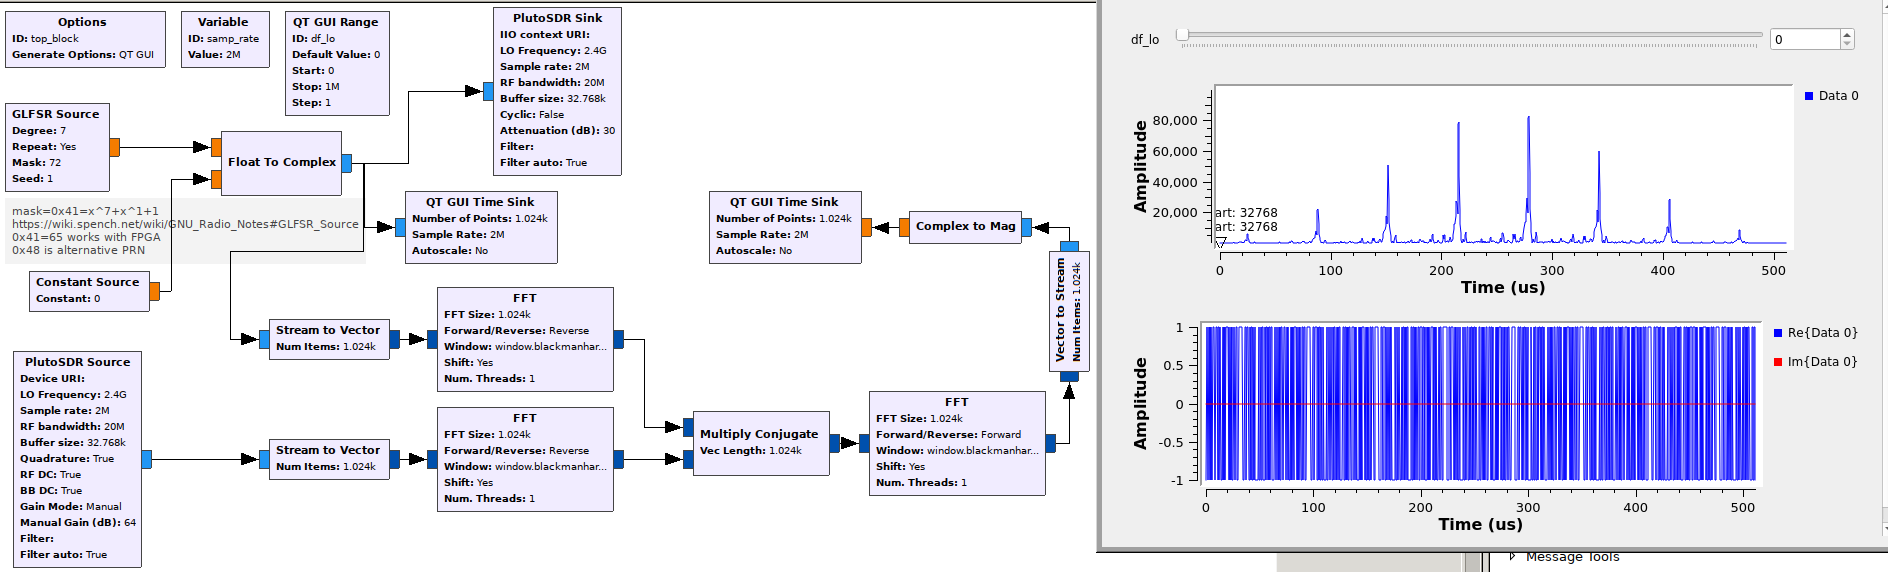
\includegraphics[width=\linewidth]{xcorr_pluto2.png}
\caption{Top: initial idea conception and experimental setup: the 10~dB attenuator
is added to try and protect the receiver from excessive emitted power but might
be omitted. Bottom: GNU Radio flowchart running the LFSR as a phase modulation of the
PlutoSDR carrier, recording the signal through the receiver and cross-correlating with
the emitted pattern to demonstrate the concept of CDMA.}
\label{f1}
\end{figure}

Again the correlation pattern (Fig. \ref{f1}, right) repeated every 127 sampling period is well visible. All these
signal processing sequences have been run on the host personal computer running GNU Radio with the PlutoSDR
fitted with the original bitstream. We now wish to run the correlation sequence on the Zynq PL and only recover
the cross-correlation output through the DataToRam interface.

The Zynq PL must be appended with two blocks: the PRN generator and the correlator. The PRN generator is
implemented as a shift register with tap positions defined by the polynomial non-zero coefficients. The feedback
is through XOR gates feeding the register input, while the PRN is observed at the output of the register.

The correlation is implemented in the time-domain which is well suited for massive parallelization on
the PL.

Remember for synthesizing the project for the PlutoSDR to export the {\tt ADI\_HDL\_DIR} variable
towards the {\tt plutosdr-fw/hdl/} directory. The {\tt design} directory hold the application
demonstration, which is compiled thanks to the provided {\tt Makefile} assuming the Vivado and
OscImpDigital variables have been set properly. Because the datastream in the PlutoSDR is clocked
at {\tt samp\_rate} (as defined by the GNU Radio flowgraph) and so is the GLFSR datastream
provided by GNU Radio Companion, the datarate will be consistent during the correlation process.
Hence, the VHDL implementation of the PRN is ({\tt fpga\_ip/prn/hdl}):

\begin{lstlisting}[language=VHDL]
--http://users.ece.cmu.edu/~koopman/lfsr/7.txt
xorM_N      <= lfsr_s(0) xor lfsr_s(6);
lfsr_next_s <= lfsr_s(BIT_LEN-2 downto 0) & xorM_N;
\end{lstlisting}
which is the straigtforward implementation of the XORed shift-register taps. The PRN generator
block can be tuned for various PRN lengths ({\tt BIT\_LEN}) and for various sequences
for this given length ({\tt PRN\_NUM}). Hence, in a CDMA demonstration approach, we can generate
two PRNs and correlate the datastream generated by GNU Radio with both sequences simultaneously:
only the matching pattern will accumulate energy in the correlation peaks and hence demonstrate
the identification process thanks to the PRN orthogonality. The cross-correlation block must
be tuned with matching sequence length: the {\tt xcorr\_prn\_slow\_complex/hdl} holds the 
implementation which states that {\tt LENGTH} is set to the PRN sequence length. 

The cross-correlation block parametrization requires defining how many correlations are run
in parallel. Due to the limited resources of the Zynq 7010 fitted on the PlutoSDR, we try to
re-use the same processing blocks as many times as possible. If the sequential processing of the
input stream becomes too long with respect ot the input stream, then parallel branches must
be used. Thus, the definition of {\tt NB\_BLK} is as follows:
\begin{enumerate}
\item let us assume an input stream at 1~Msamples/s, and the internal clock rate of the PlutoSDR
of 100~MHz
\footnote{
FCLK\_CLK0 of sys\_ps7 block is defined as shown by double clicking on the block
and selecting Clock Configuration $\rightarrow$ PL Fabric Clock $\rightarrow$ FCLK\_CLK0=100~MHz.
This information is initially defined in the TCL script {\tt system\_bd.tcl} as
{\tt ad\_ip\_parameter sys\_ps7 CONFIG.PCW\_FPGA0\_PERIPHERAL\_FREQMHZ 100.0}}. 
Then a single cross-correlation {\tt xcorr\_prn\_slow\_complex} can process 
100~correlations before a new input bit is clocked by the datastream
\item one last processing block is always assumed to be added to process the remaining number
of samples. In this case, 27 more correlations will be needed, which can be performed by this
second implicit processing block (since $27<100$)
\item if the clock had only been 50~MHz, then 2~blocks would have been needed: the two blocks
would have processed $2\times 50=100$~correlations sequentially, and the remaining 27 could have
been taken care of by the additional implicit block since $27<50$.
\end{enumerate}

Hence, the TCL file defining the PlutoSDR firmware is appended ({\tt design/system\_bd.tcl}) with
\begin{lstlisting}[language=TCL]
# prn1
ad_ip_instance prn prn1_gen
ad_ip_parameter prn1_gen CONFIG.PERIOD_LEN 1
ad_ip_parameter prn1_gen CONFIG.BIT_LEN 7
ad_ip_parameter prn1_gen CONFIG.PRN_NUM 1

ad_connect sys_ps7/FCLK_CLK0 prn1_gen/clk
ad_connect sys_rstgen/peripheral_reset prn1_gen/reset

# xcorr1
ad_ip_instance xcorr_prn_slow_complex xcorr1
ad_ip_parameter xcorr1 CONFIG.LENGTH 127
ad_ip_parameter xcorr1 CONFIG.NB_BLK 1
ad_ip_parameter xcorr1 CONFIG.IN_SIZE 16
ad_ip_parameter xcorr1 CONFIG.OUT_SIZE 32

ad_connect duppl_xcorr/data1_out xcorr1/data_in
ad_connect prn1_gen/prn_o xcorr1/prn_i
ad_connect xcorr1/prn_sync_o prn1_gen/tick_i

#dataComplex
ad_ip_instance dataComplex_to_ram data_to_ram
ad_ip_parameter data_to_ram CONFIG.NB_INPUT 1
ad_ip_parameter data_to_ram CONFIG.DATA_SIZE 32
ad_ip_parameter data_to_ram CONFIG.NB_SAMPLE 2048

ad_connect xcorr1/data_out data_to_ram/data1_in
ad_connect sys_rstgen/peripheral_reset data_to_ram/s00_axi_reset

ad_cpu_interconnect 0x43C20000 data_to_ram
\end{lstlisting}
defining the first ({\tt PRN\_NUM}) sequence of PRN with 127-length ({\tt BIT\_LEN}) clocked
by the internal 100~MHz clock ({\tt sys\_ps7/FCLK\_CLK0}) and the cross correlation
operates on these 127-bits ({\tt LENGTH}) with a single processing block ({\tt NB\_BLK}) considering
than an implicit second block will take care of the remaining 27~cycles.

\begin{figure}[h!tb]
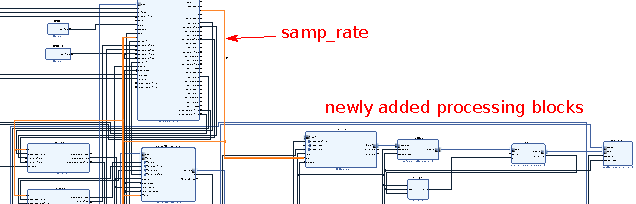
\includegraphics[width=\linewidth]{1xcorr_1PRN_crop.pdf}
\caption{PRN generator and cross-correlation with the received datastream.}
\label{ex1}
\end{figure}

We see on this TCL script -- or in Vivado by double-clicking on the Data\_to\_RAM block, that the
data size will be encoded as 32-bit words. Since we are handling complex data, we fetch two 32-bit 
words for each sample, and a total of 2048 samples are stored in the RAM. Hence, the userspace
application for fetching the data will be
\begin{lstlisting}[language=C]
int main()
{int32_t c[2048 * 2 *NUM_PRN]; /* two input (x2) x 2048 sample complex (x2) */
 int fi, fo;
 fi = open("/dev/data3200", O_RDWR);
 fo = open("/tmp/data.bin", O_WRONLY | O_CREAT);
 read(fi, c, 2048 * 2 * NUM_PRN * sizeof(int32_t));
 write(fo, c, 2048 * 2 * NUM_PRN * sizeof(int32_t));
 close(fi);
 close(fo);
}
\end{lstlisting}
and the resulting {\tt /tmp/data.bin} is transfered to the host PC for reading by GNU/Octave (Fig. \ref{res1})
with \\{\tt fd=fopen("data.bin"); a=fread(fd, Inf, "int32"); prn=a(1:2:end)+i*a(2:2:end); plot(abs(prn1));}.

\begin{figure}[h!tb]
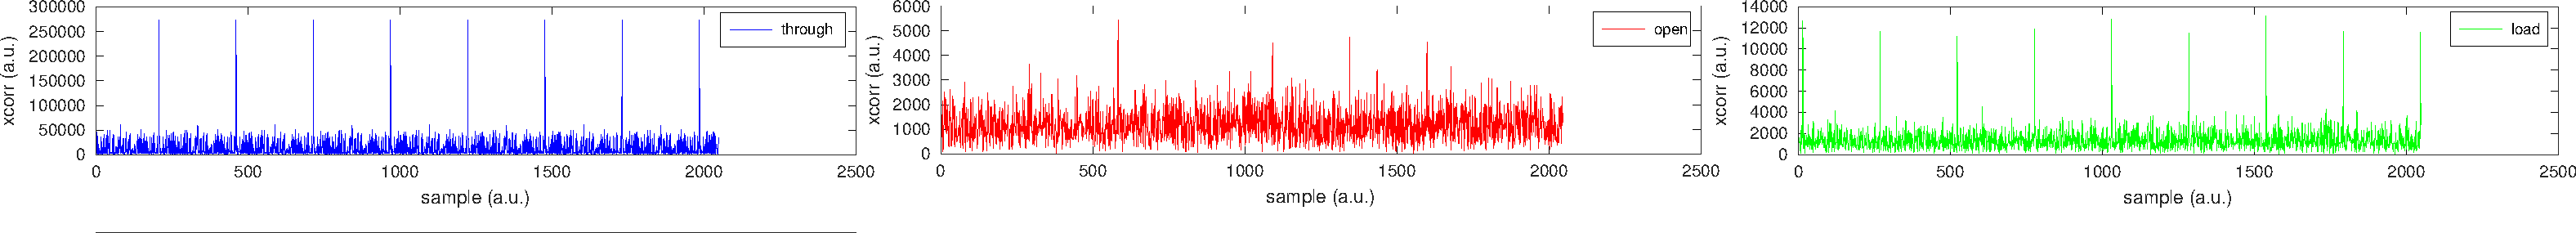
\includegraphics[width=\linewidth]{results/example1.pdf}
\caption{Correlation output from the PL processing, left to right with a through connexion
between TX and RX, open circuit or loaded input and output (50~$\Omega$).}
\label{res1}
\end{figure}

The last challenge is the different datarates between the PRN generation and the cross-correlator.
Indeed the cross-correlator is clocked by the 100~MHz AXI bus clock while the input datastream
is clocked at the {\tt samp\_rate} rate. Hence, a FIFO block must be included between the 
output datastream and the cross correlator input (Fig. \ref{ex1}).

Since the 7-bit PRN generator is designed to only generate one pseudo-random sequence out of the 
18 possible options (\url{http://users.ece.cmu.edu/~koopman/lfsr/7.txt}), namely the taps defined 
as 0x41=65 (or $x^7+x^6+1$), we can also use this opportunity to demonstrate the orthogonality of 
the codes needed for CDMA. Indeed cross correlating to null-mean value pseudo-random sequence will 
not allow for coherent energy accumulation and will not yield discrete correlation peaks when 
the two sequences match.

\begin{figure}[h!tb]
% 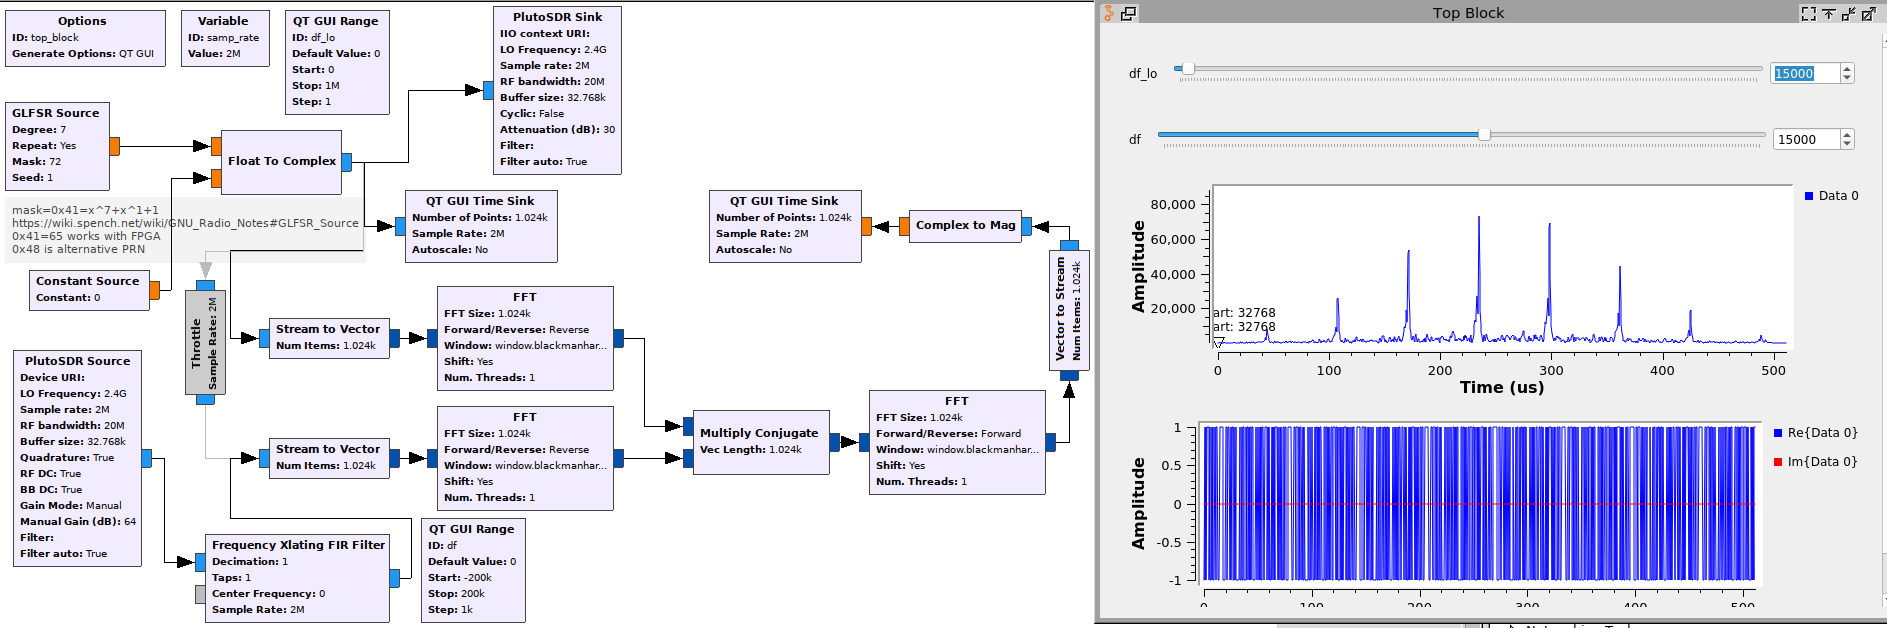
\includegraphics[width=\linewidth]{xcorr_pluto3g.png}
\caption{Running the same PRN sequence on the Zynq PL (receiver side) than the one emitted by 
GNU Radio
allows for identifying cross-correlation peaks separated by the PRN length of 127 samples. Emitting a
different PRN sequence than the one run on the Zynq PL yield close-to-zero cross correlations, hence
demonstrating the orthogonality of PRN codes.}
\label{f2}
\end{figure}

\section{7-bit PRN on different receive and transmit carrier frequencies}

We are convinced the correlator block is operational and fits in the PL remaining resources (although
decoding 1023-bit long GPS Gold Codes will require extending the correlator length from 127 to 1023 bits,
hence using more resources), and that we understand how to generate PRN sequences matching incoming patterns.

\begin{figure}[h!tb]
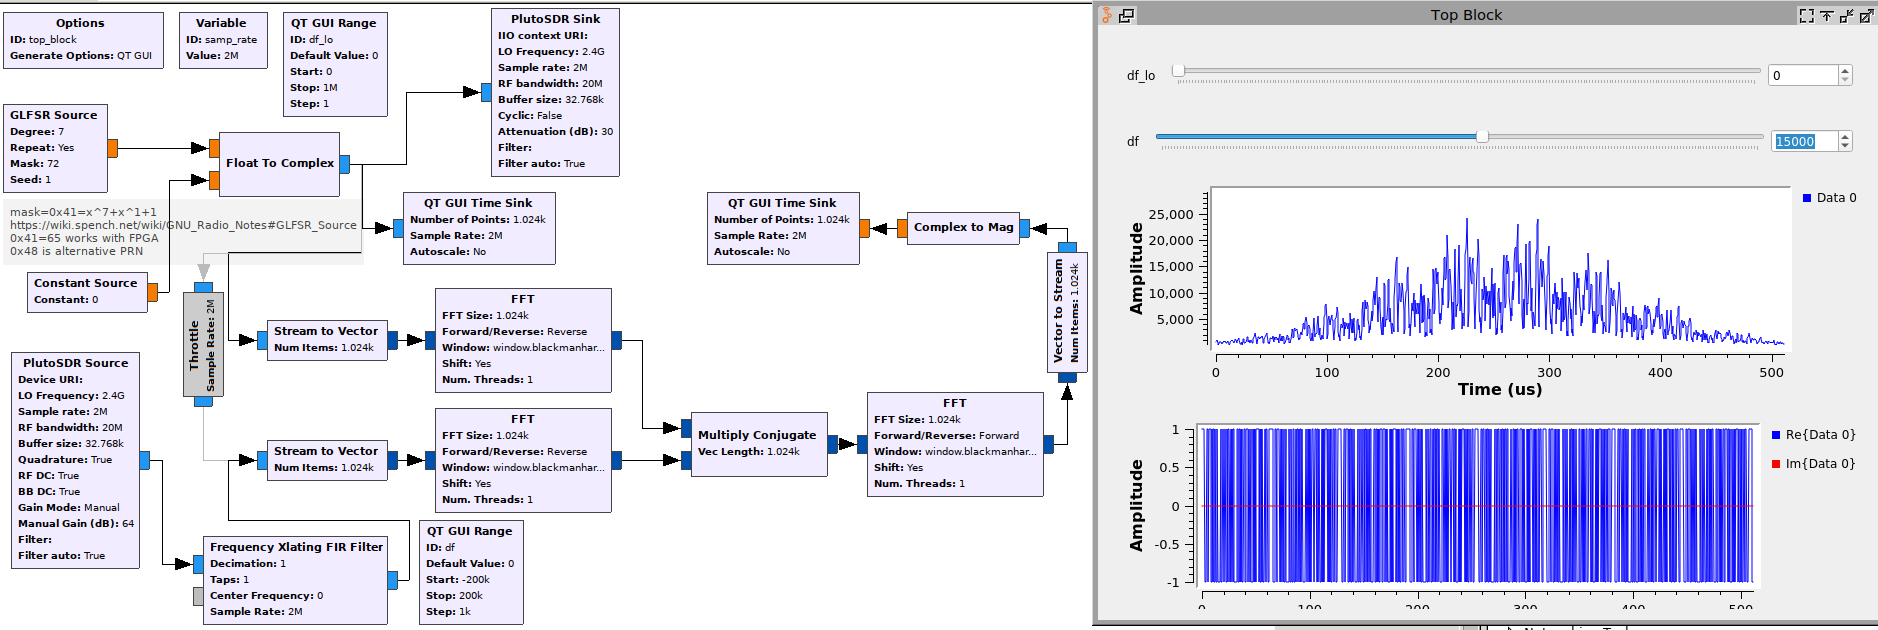
\includegraphics[width=\linewidth]{xcorr_pluto3ng.png}
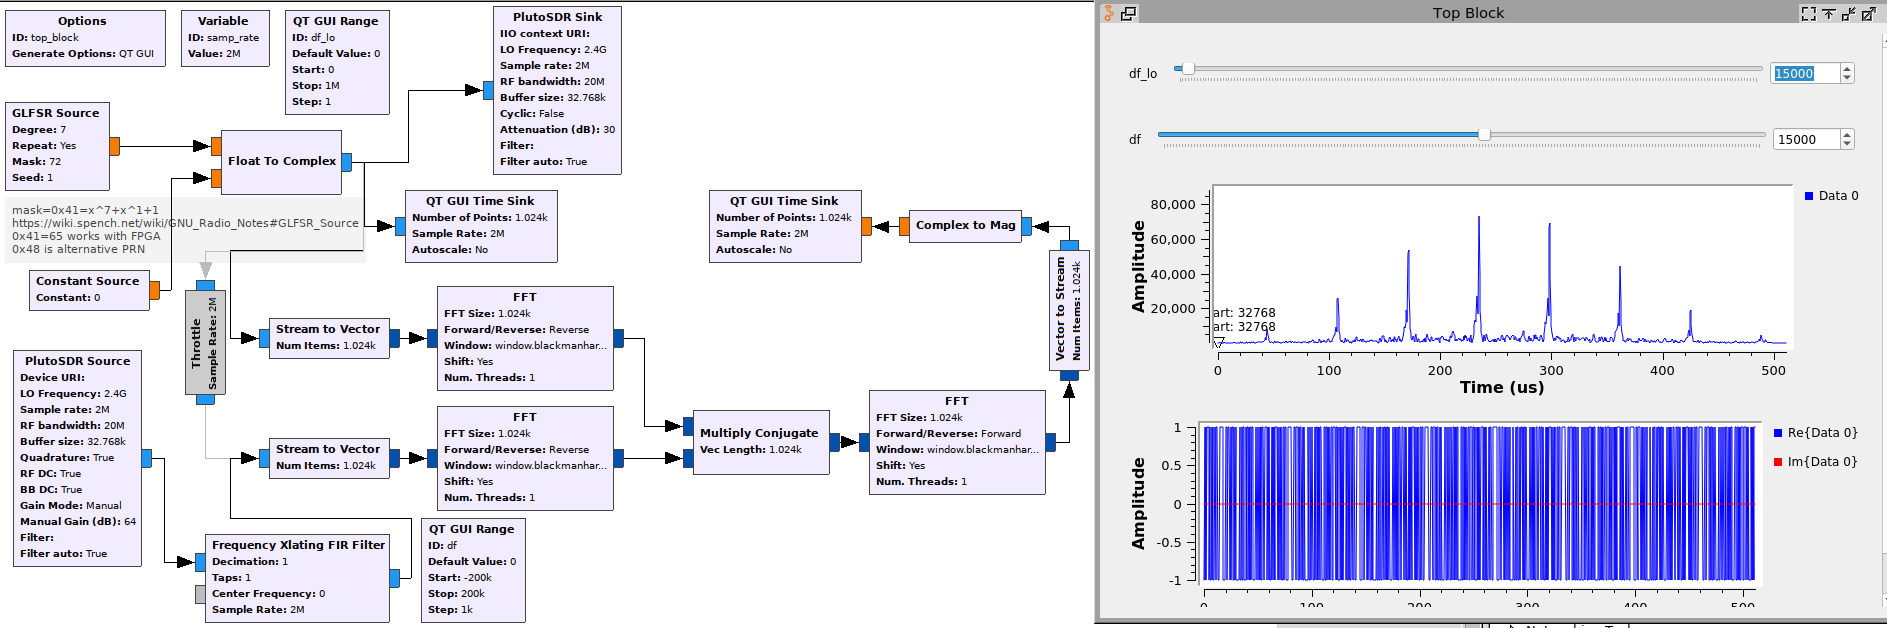
\includegraphics[width=\linewidth]{xcorr_pluto3g.png}
\caption{Offsetting the emitted frequency with respect to the received frequency (top) prevents
the cross-correlation from accumulating energy due to the null mean power of the trigonometric
functions. Compensating for the frequency offset solves the issue (bottom), as will be needed
in the case of GPS reception due to the Doppler frequency shift associated with satellite motion.}
\label{f3}
\end{figure}

However, GPS satellites are not geostationary but moving along their orbit at an altitude of 20000~km. Basic
celestial mechanics tells us that the period is 12~hours, and dividing the orbit length by the period gives
us the satellite velocity from which the Doppler shift is deduced. We expect Doppler shifts in the $\pm 5$~kHz 
range, while the cross-correlation of the 1023-bit long code running at 1.023~Mb/s will be canceled for
any frequency offset of more than 1~kHz (inverse of 1~ms repetition rate) due to the zero-mean value of trigonometric
functions. Practically, good signal to noise ratio will be achieved if the receiver frequency is not offset
by more than 500~Hz from the emitter frequency. Hence, Doppler shift compensation on the receiver side is needed:
the {\bf acquisition} phase of GPS reception means sweeping all possible Space Vehicle (SV$\in[1..32]$) code and 
all possible Doppler frequency shifts to try and find which satellite is at what position. This step will be 
addressed in this document, while the following {\bf tracking} phase will not be addressed.

Back to basics, we wish to demonstrate on the 7-bit long PRN sequence how a frequency offset between emitter
and receiver can be compensated for by including a PS-configurable Numerically Controlled Oscillator (NCO) and
mixing the incoming signal prior to correlating. Again we first start demonstrating the concept using GNU Radio
prior to extending the demonstration to the Zynq PL. Fig. \ref{f3} demonstrates using GNU Radio's Frequency 
Xlating FIR Filter to compensate for the frequency offset introduced on purpose between the PlutoSDR emitter and 
receiver. Fig. \ref{f3} indeed demonstrates that the correlation remains null for high frequency offsets and
that the correlation peaks re-appear once the frequency offset has been compensated for.

The challenge of implementing the NCO in the FPGA is that we must know what the sampling frequency is, {\em i.e.}
know the clock rate of the NCO block. We have identified that the frequency of the signal propagated in the 
FPGA is given by reading\\
{\tt /sys/bus/iio/devices/iio\:device1/in\_voltage\_sampling\_frequency}\\
which tells us that the GNU Radio {\tt samp\_frequency} is the clock signal frequency in the PL.

% {\bf TODO: describe NCO and complex mixer}
The PL implementation is quite similar except that this time the NCO must be included
between the datastream -- running at {\tt samp\_rate} -- and the FIFO feeding the correlator (Fig.
\ref{ex2}).

\begin{figure}[h!tb]
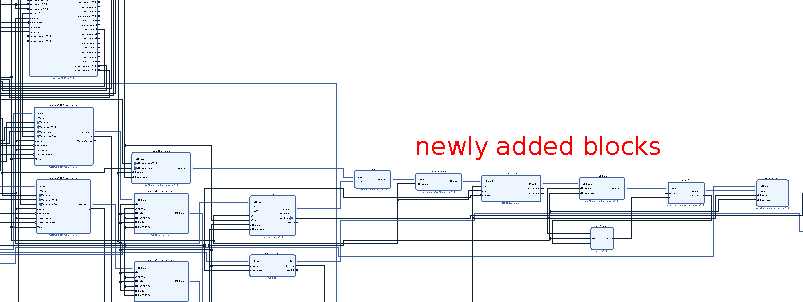
\includegraphics[width=\linewidth]{1xcorr_1PRN_NCO_crop.pdf}
\caption{PRN generator and cross-correlation with the received datastream with frequency
transposition using the NCO.}
\label{ex2}
\end{figure}

In order to demonstrate both frequency shifting capability and dual-PRN detection to select
one emitter or the other, two PRN generators and two correlators can be included in the
decoding path (Fig. \ref{ex3}).

\begin{figure}[h!tb]
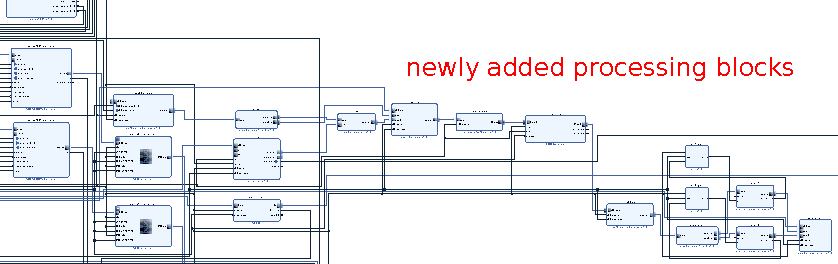
\includegraphics[width=\linewidth]{2xcorr_2PRN_NCO_crop.pdf}
\caption{Dual PRN generator and cross-correlation with the received datastream frequency
transposed using the NCO.}
\label{ex3}
\end{figure}

\section{GPS signal reception}

The knowledge acquired so far now allows us to tackle GPS acquisition. During this
initialization phase in which the receiver does not know what its local oscillator offset is,
which satellite is visible and where they are located in the sky, a brute force approach is needed
to try all possible satellite identifiers with all possible Doppler shifts\footnote{the receiver
can actually get a hint of the Doppler shifts to be investigated by squaring the BPSK signal
and looking at the spectral components of the Fourier transform of the resulting signal. Since
squaring a BPSK modulated signal gets rid of the modulation, strong spectral components will be
visible at twice the offset frequency.}. Hence, the NCO is programmed with narrow enough frequency
steps to sweep all possible Doppler shifts, and all possible space vehicle PRNs are correlated
with the frequency transposed I/Q signal. GPS does not use a basic 10-bit long PRN but the so-called
Gold code provided in the {\tt cacode} FPGA IP. Notice that this same function is available for
Matlab or GNU/Octave at \url{https://www.mathworks.com/matlabcentral/fileexchange/14670-gps-c-a-code-generator}
and will be used later in the software-decoding of GPS.

The first step is to assess the hardware setup and being able to collect I/Q streams using the 
PlutoSDR tuned to the GPS carrier frequency of 1575.42~MHz (Fig. \ref{f4}). Since our NCO only accepts positive
frequencies, we actually slightly offset the carrier frequency so that the Doppler correction is
achieved only by programming positive frequencies when configuring the NCO.

\begin{figure}[h!tb]
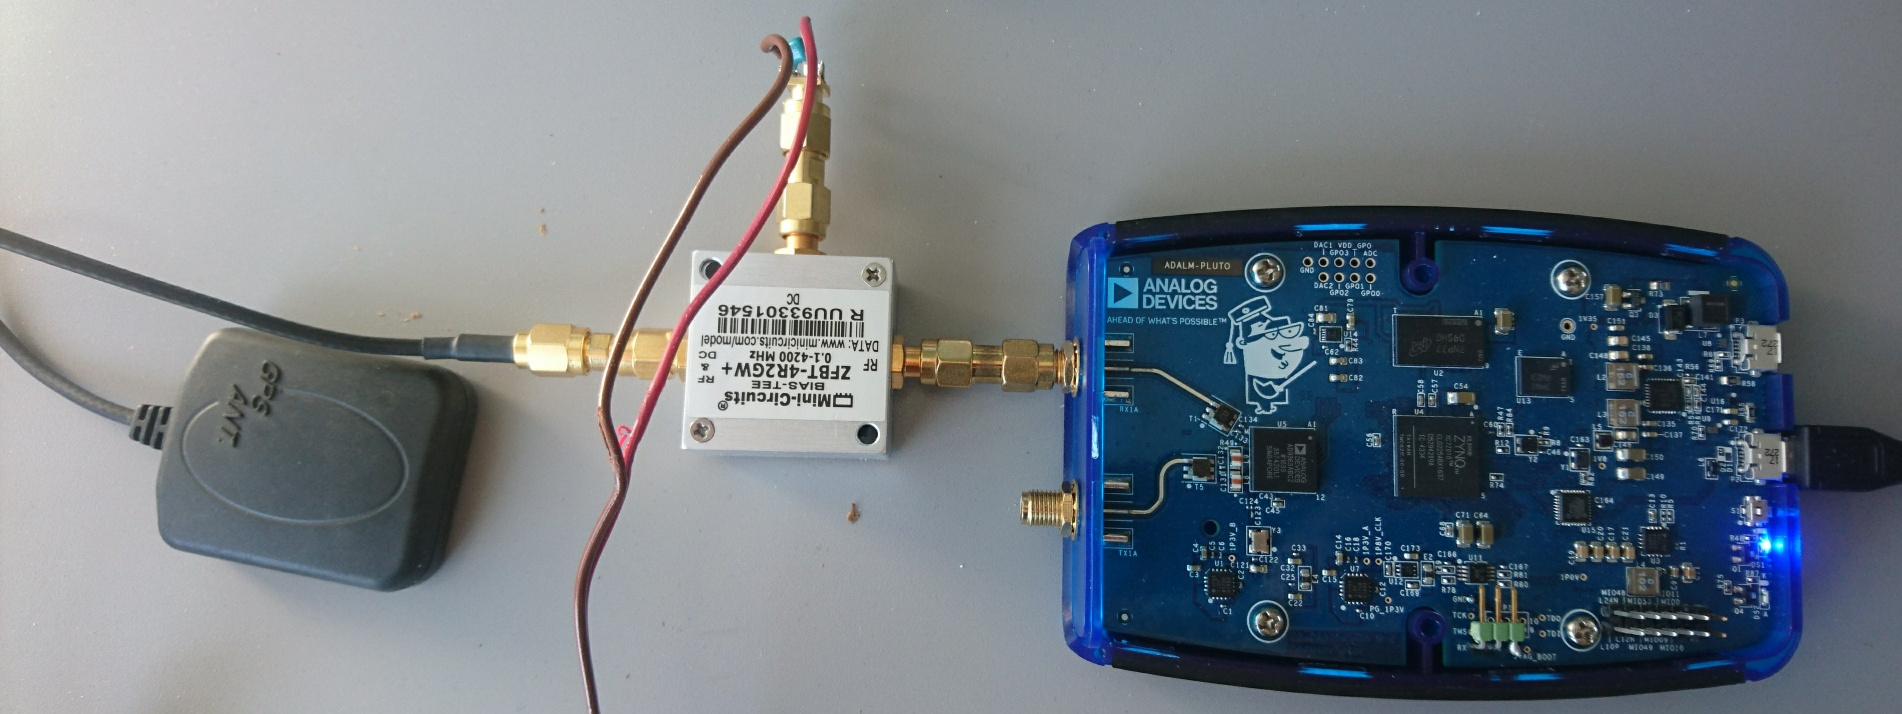
\includegraphics[width=\linewidth]{DSC_0279.JPG}
\caption{Experimental setup: a bias-T is introduced between the PlutoSDR RX input and the
GPS antenna to power the antenna amplifier. A radiofrequency-grade 1 to 100~$\mu$H inductor
connected to the +5~V power supply and a 1~nF capacitor to the receiver will provide similar 
results.} 
\label{f4}
\end{figure}

While {\tt cacode} outputs all SV sequences, the space available on the Zynq-7010 of the PlutoSDR only
allows for synthesizing a single cross-correlating block for 1023-bit long sequences. Hence, the
Zynq PS is programmed to configure a single SV identifier, and then sweep NCO values. Since the 
1023-bit long is run at 1.023~Mb/s on the GPS satellite, the code repeats every millisecond. To make
sure we observe a fine correlation peak, we sweep the frequency with 300~Hz steps.

\begin{figure}[h!tb]
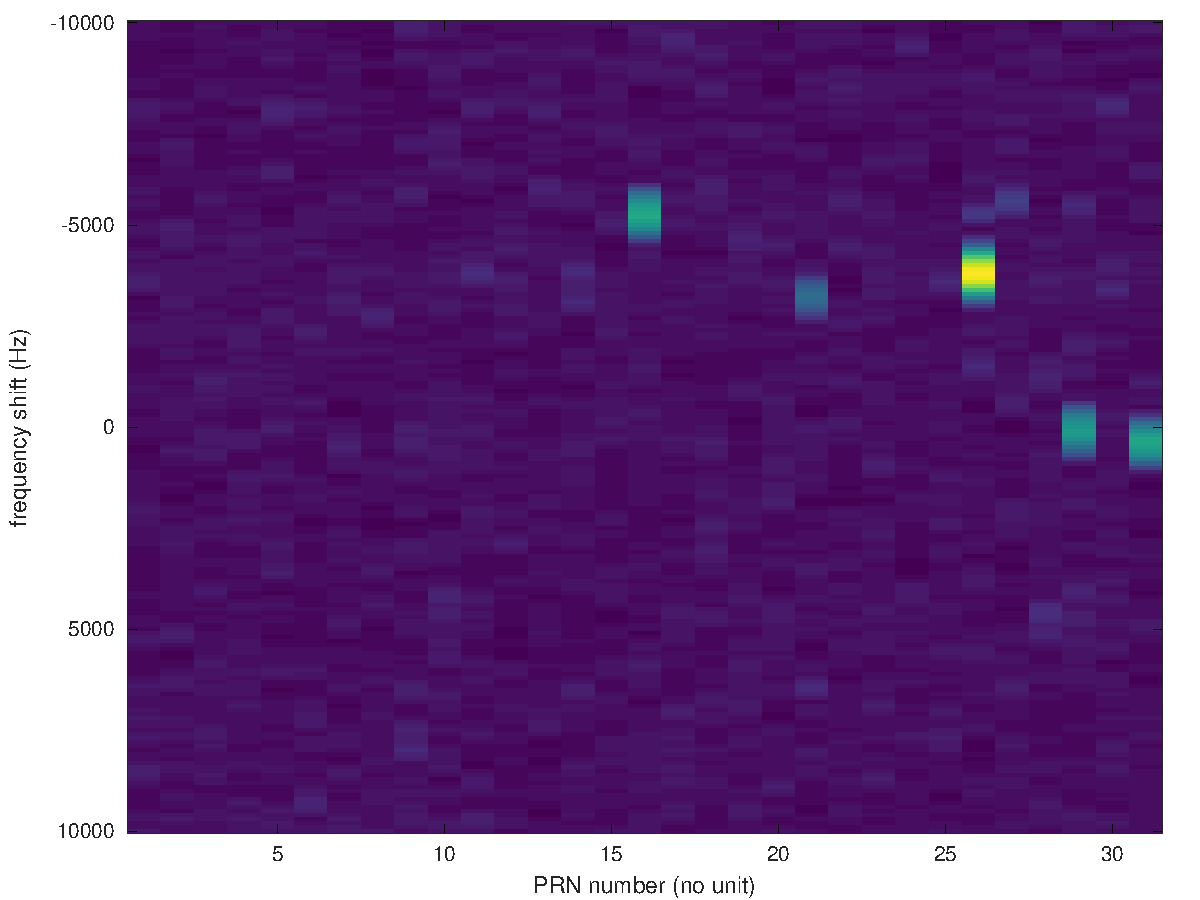
\includegraphics[width=.49\linewidth]{190524gps_xcorr/gps_bin100Hz.pdf}
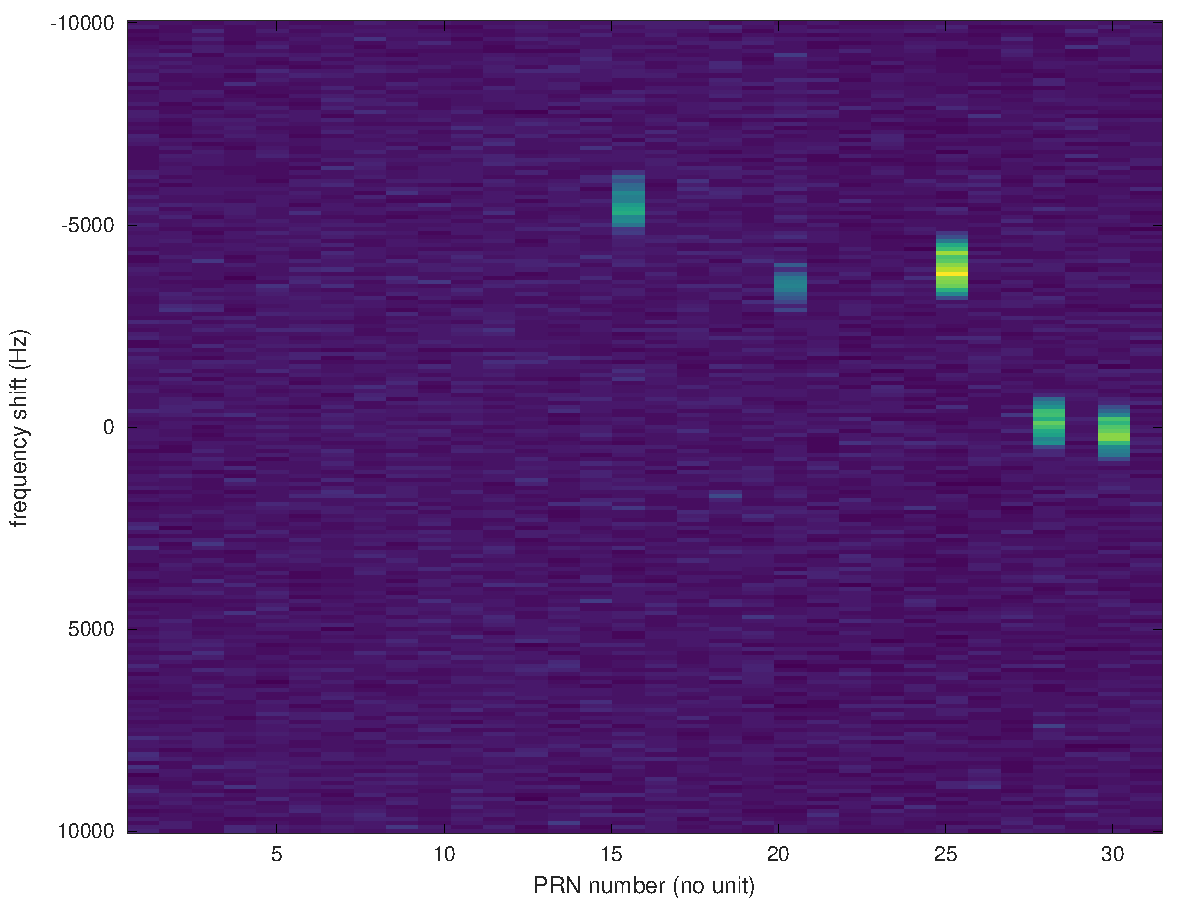
\includegraphics[width=.49\linewidth]{190524gps_xcorr/gps_plutosdr.pdf}
\caption{Left: cross-correlation (color code) maximum as a function of SV number (abscissa) and frequency
offset (ordinate) as computed using GNU/Octave on a 250~ksamples record collected from the
PlutoSDR. Right: same computation as performed on the Zynq PL. The results are consistent with space
vehicles 16, 21, 26, 29 and 31 clearly visibles at frequency offsets within the $\pm$5~kHz range expected
from the Doppler shift. No local oscillator bias is seen on this PlutoSDR.}
\label{f5}
\end{figure}

Running all SV identifiers and for each SV, running all frequency offsets in a $\pm 100$~kHz range (to account
for possible local oscillator bias) requires 1 minute and 50 seconds for 100~Hz steps and 31 satellites
(Fig. \ref{f5}, bottom right) or 36 seconds for 300~Hz steps. Mapping the constellation of satellites
with 500~Hz steps (Fig. \ref{f5}, bottom left) is hence expected to require only 22~seconds when running on
the computation on the PL. The same computation result (500~Hz steps, 31 satellites) requires 108 seconds
on a 2.60~GHz i5-3320M CPU as found in the Panasonic CF-19 running GNU/Octave, while the displayed chart
(100~Hz steps) required 504~seconds using the following program:
\begin{lstlisting}[language=octave]
pkg load signal
x=read_complex_binary('./gps.bin');
fs=1.023; % MHz                   % sampling frequency
freq0=[-1.0e4:500:1.0e4]-20000;   % frequency range
x=x(1:2e5);                       % data subset
time=[0:1/fs/1e6:length(x)/fs/1e6]';time=time(1:end-1); % discrete time
for m=[1:31]                      % PRN number
   a=cacode(m,fs/1.023); a=a-mean(a);
   l=1; m
   for freq=freq0                 % run through possible frequency offsets
    mysine=exp(j*2*pi*(-freq)*time); 
    xx=x.*mysine;                 % frequency shift the signal
    [u(l,m),v(l,m)]=max(abs(xcorr(a,xx))); % check for cross correlation max.
    l=l+1;
   end
end
imagesc([1:31],-freq0-20000,abs(u))
\end{lstlisting}

\begin{thebibliography}{9}
\bibitem{collins} T.F. Collins, R. Getz, D. Pu \& A.M. Wyglinski, {\em Software-Defined 
Radio for Engineers}, Artech House (2018), p.171 at
\url{www.analog.com/en/education/education-library/software-defined-radio-for-engineers.html}
\end{thebibliography}
\end{document}
